
\documentclass[letterpaper]{article}
\usepackage{aaai}
\usepackage{times}
\usepackage{helvet}
\usepackage{algorithm}
\usepackage{algpseudocode}
\usepackage{courier}
\usepackage{graphicx}
\graphicspath{{./figure/}}
\frenchspacing
\setlength{\pdfpagewidth}{8.5in}
\setlength{\pdfpageheight}{11in}
\begin{document}    

\section{Implementation}
We implemented our method and applied it to the Angry Birds where the vision can detect the exact shapes of the objects\cite{}. The objects' visual appearance are restricted to a finite number of templates (See Figure \ref{Templates}).

The vision has the following limitations: 1) Damaged objects will be detected as a few separate smaller pieces. (Figure \ref{Fragments}.b) 2) Debris are not recognized so that one cannot determine whether an object, say a stone, is a real stone or just a debris from a previously destroyed stone. (Figure \ref{Fragments}.a) 3) Objects occlusion is not handled. Objects can be partially or entirely occluded by debris or other game effects e.g. prompted scores or clouds around the hit point (See Figure \ref{Fragments}.c)

We show those problem can be dealt with effectively by the above mentioned techniques.

\begin{figure}[h!]
\centering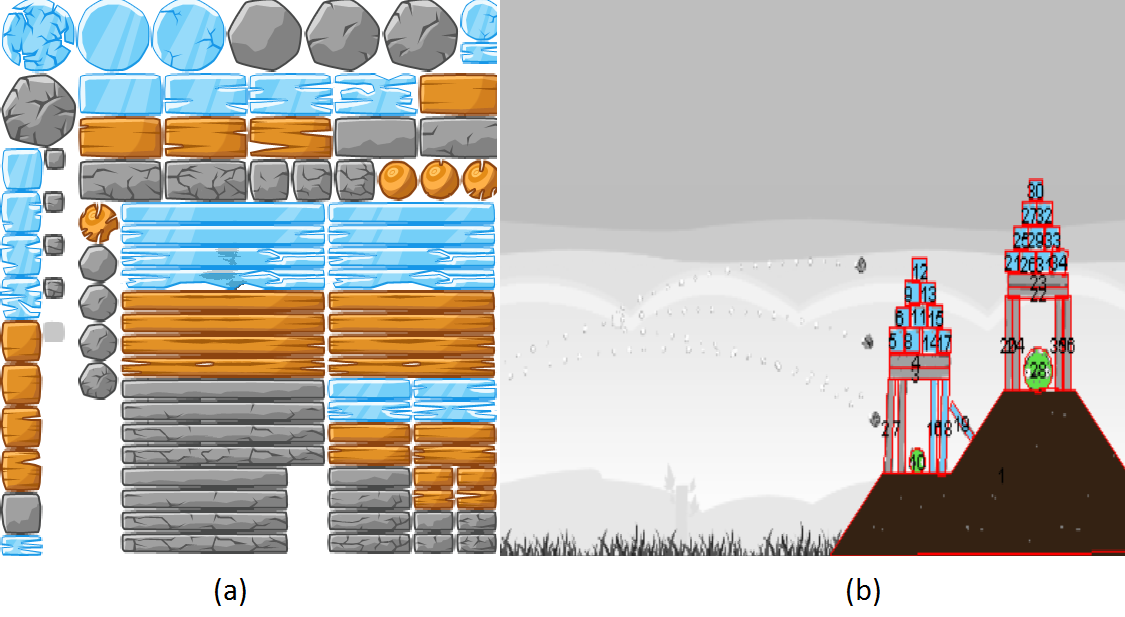
\includegraphics[scale=0.28]{Templates.png}\caption{(a) Main Templates used in Angry Birds (b) The vision detects the real shapes of the objects in a typical Angry Birds scenario}
\label{Templates}
\end{figure}


\begin{figure}[h!]
\centering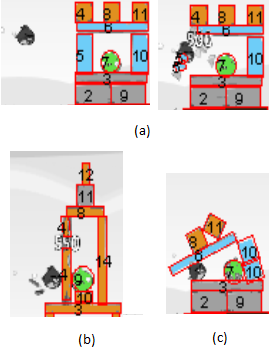
\includegraphics[scale=0.7]{Fragmentation.png}\caption{(a) An object (ID 5) is broken into pieces by a hit (b) An object (ID 4) is partially occluded (c) An object (ID 10) is damaged and detected as two separate blocks}
\label{Fragments}
\end{figure}

\subsection{Handling Fragmentation and Occlusion}

Objects fragmentation creates new objects in subsequent images and the new objects are not directly related to the initial objects. The varying number of objects from one scenario to another can introduce ambiguities making a tracking algorithm off the track. 

In angry birds, the fragmentation is mainly due to objects destruction, partially occlusion, and damage. Handling fragmentation is important. By recognizing the fragments, we are able to infer whether an object is destroyed, damaged, or occluded, which leads to a robust tracking.

We deal with the fragmentation by first recognizing potential fragments, then construct all the possible objects from the fragments, and add them to the pool of the subsequent objects for matching, and finally apply a debris recognition process for the unmatched initial objects. 

To obtain the potential fragments, we group the initial and subsequent objects according to their templates, respectively. If a group of the subsequent objects contains more objects than its initial counterpart, we treat all those subsequent objects as potential fragments.  

For all the potential fragments, we put those that can form a shape of one of the templates into a same group. The shape formed by the group of fragments is an oriented minimum bounding rectangle (OMBR) that bounds all the fragments (see Figure \ref{OMBRs}.a). The fragments from one group must have the same type. We then treat the OMBR as one object in the subsequent image, which can be potentially matched with one of the initial objects. Once the OMBR is matched, all the fragments from the corresponding group are also matched. i.e. assigned with the same ID. In some rare cases, a fragment can be involved in more than one OMBRs. So we add an additional constraint: all the matched OMBRs should not have a common fragment. 

We label unmatched fragments as debris. Destruction of an object will create a cluster of debris around the object's location. Those debris can be of any shape, e.g. circle, polygon and will diffuse until disappear after 2-4 seconds. Given an object $o$ in the initial scenario, we start the debris recognition process if there are no subsequent objects can be matched with $o$ (including the OMBRs created from the fragments). We first draw the MBC of $o$, and get the set of the subsequent objects falling in the MBC excluding those which have been matched. The set of the objects are labelled as debris of $o$ and $o$ is marked as destroyed (see Figure \ref{OMBRs}.b). 

In some cases, an object can be totally occluded for a subsequence of images. To deal with this, before a matching, we cache the spatial configurations of all the initial objects. At the end of the matching, we update the cache by replacing each initial object's configuration with the matched subsequent object's so that the cache always maintains the latest configuration of each initial object. If an occluded object recurs in one subsequent image, we match the occluded object by searching through the cache for an unmatched initial object. The occlude object will be matched if it lies in the MBC of that initial object. 


\begin{figure}[h!]
\centering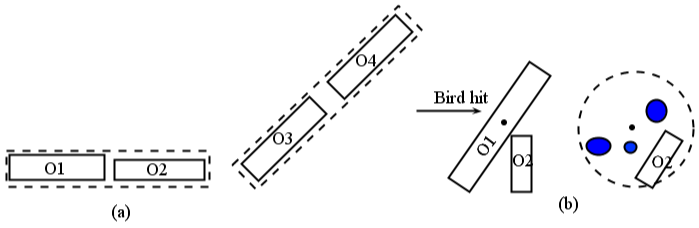
\includegraphics[scale=0.3]{OMBRs.png}\caption{(a) OMBRs are indicated by the dotted rectangles (b) $o_1$ has been destroyed by a bird hit, and the blue dots are recognized as debris}  
\label{OMBRs}
\end{figure}



\end{document}